%---------------------------------------------------------------------
%   pdf para imprimir o contido
%---------------------------------------------------------------------
\documentclass[twoside,a4paper]{article} 		% non deixa amsart   twocolumn,
\usepackage[spanish,galician]{babel}
\usepackage[utf8]{inputenc}
%---------------------------------------------------------------------------------------------
 %  Paquete para que faga artigo dende algo que ten a pinta beamer
 %---------------------------------------------------------------------------------------------
\usepackage{beamerarticle}
     
%----------------------------------------------------------------------------------------------------------------
% Tells the beamer class where to  find the presentation version of the current file.
%----------------------------------------------------------------------------------------------------------------     
\setjobnamebeamerversion{main.beamer}

%---------------------------------------------------------------------------------------------------------------- 
% Cabeceira e pe de páxina
%---------------------------------------------------------------------------------------------------------------- 
\usepackage{lastpage}
\usepackage{fancyhdr}
\pagestyle{fancy} 
\fancyhf{}
\fancyhead[RE,LO]{ 
\includegraphics[width=\linewidth,width=2cm]{debuxos/i-rocho.png} }
\fancyhead[LE,RO]{\scshape \scriptsize \titulito}
\cfoot{\scshape \small Páxina \thepage ~de~ \pageref{LastPage}}
\renewcommand{\headrulewidth}{0.1pt}

%----------------------------------------------------------------------------------------------------------------
% Pinta no folio
%---------------------------------------------------------------------------------------------------------------- 
%   Interespaciado
\renewcommand{\baselinestretch}{1}
\linespread{2}

%% Marxes
\usepackage[a4paper]{geometry}
\newgeometry{top=2cm,left=2cm,right=2cm,bottom=2cm}   


%---------------------------------------------------------------------
% Lista de paquetes ó mogolón
%---------------------------------------------------------------------
%---------------------------------------------------------------------------------------------
 %  Paquetería común 
  %---------------------------------------------------------------------------------------------
\usepackage[spanish,galician]{babel}
\usepackage[utf8]{inputenc}
\usepackage{graphicx}
\usepackage{epsfig} 	% for figures
\usepackage{xcolor} 	% for color
\usepackage{amssymb,amsmath}
\usepackage{wrapfig}
\usepackage{setspace}
\usepackage{multicol}
\usepackage{fancybox}
%Simple ou dobre columna
 \usepackage{multicol}
%ligazóns
\usepackage{hyperref}	

\date{}
\author{http://irocho.wordpress.com}

%---------------------------------------------------------------------
% Título chulo con logo
%---------------------------------------------------------------------
\title{ \raggedright
  
\includegraphics[width=\linewidth,width=4cm]{debuxos/i-rocho.png} 
    \\
    \centering 
    \titulito
    }

%%-------------------------------------------------------------------
% Para poder facer \begin{diapo}...\end{diapo}
%---------------------------------------------------------------------
\newenvironment{diapo}
{	
	%\vspace{0.5cm}  				%ou queda pegañado ó texto
	\linespread{1}
	\sffamily						%respostas en sans serif
	\noindent 	
	\begin{Sbox}					%comeza facer recadro
	\begin{minipage}[t]{0.48\textwidth} 	%recadro ocupa a metade 
}
{
	\end{minipage}
	\end{Sbox}\shadowbox{\TheSbox}		%pinta recadro sombreado
	%\vspace{0.2cm}						%ou queda pegañado ó texto
}



%---------------------------------------------------------------------
%Trae o contido: o dos frame e o de fóra
%---------------------------------------------------------------------
%---------------------------------------------------------------------------------------------
 %  Contido :
 %        diapos con:  \begin{diapo}..... \end{diapo}
 % 	    texto que vai saír por impresora: fóra dos frame
 %        notas íntimas que podo imprimir á parte \note{}
 %---------------------------------------------------------------------------------------------
 
% Lembrar non \documentclass.... 

%---------------------------------------------------------------------------------------------
 %  Paquetería común 
  %---------------------------------------------------------------------------------------------
\usepackage[spanish,galician]{babel}
\usepackage[utf8]{inputenc}
\usepackage{graphicx}
%\usepackage{epsfig} 	% for figures
%\usepackage{xcolor} 	% for color
%\usepackage{amssymb,amsmath}

%   Simple ou dobre columna
 \usepackage{multicol}

%ligazóns
\usepackage{hyperref}	

%----------------------------------------------------------------------------------------------------------------
%  Títulos
%---------------------------------------------------------------------------------------------------------------- 
\newcommand{\titulito}{
Caracterización de Sistemas Operativos
}
\subtitle{
Cuestións sen resposta en contexto
}
\newcommand{\asignatura}{
Sistemas Operativos Monoposto
%Montaxe e Mantemento
}


\begin{document}
%----------------------------------------------------------------------------------------------------------------
%  Títulos segundo o tipo de documento
%---------------------------------------------------------------------------------------------------------------- 
\mode <beamer>{
\begin{frame}
\maketitle
\end{frame}
}
% o título queda máis chulo sen ser a dúas columnas
\mode <article>{
\maketitle
}
%----------------------------------------------------------------------------------------------------------------
% Contido
%---------------------------------------------------------------------------------------------------------------- 
%\abstract{			}%sae no main. article

\begin{wrapfigure}{r}{0.5\textwidth}
	\begin{center}
	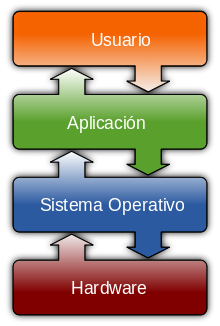
\includegraphics[width=0.2\textwidth]{./debuxos/capas.png}
	 \caption{Situación do sistema operativo}
	 \end{center}
	 \label{capas}
\end{wrapfigure}

\begin{doublespace}
Nos anos corenta cando se comezaron a construír ordenadores os programadores tiñan que ter en conta as peculiaridades do equipo co que traballaban. Non era o mesmo programar para un procesador ou para outro, as instrucións tiñan que indicar por exemplo o espacio de memoria que se ía usar. Co paso do tempo foron decatándose de que era mellor ter un software que se ocupara dos detalles de máquina e que o programador poidera executar o seu código en calquera equipo. Precisaban un software que se encargara dos detalles concretos do ordenador: do espacio libre en memoria, das instrucións que variaban dun procesador a outro, de verificar se todo funcionaba correctamente,... Paseniño foise creando ese software que permite ó programador ocuparse do seu cálculo ou do seu algoritmo sen ter que preocuparse en que parte da memoria se executa ou cal é o procesador que lle está resolvendo as súas contas. 

Un sistema operativo é ese conxunto de programas que actúan coma intermediario entre o usuario e o hardware do ordenador. Na figura \ref{capas} vemos como o sistema operativo sitúase facendo de intermediario entre os dispositivos físicos e as aplicacións de usuario.\\
\end{doublespace}

\begin{diapo} \begin{frame}{Un sistema operativo é  \dots} 
\begin{enumerate}
\item hardware\pause
\item software \pause
\item malware 
\end{enumerate}
\end{frame} 
\end{diapo} 
%parella
\begin{diapo}\begin{frame}{Os que xestionan o hardware son  \dots}
\begin{enumerate}
\item drivers \pause
\item terminais \pause
\item sistemas operativos
\end{enumerate}
\end{frame}
\end{diapo}



\newpage

\section{Funcións dun sistema operativo}
Hoxe en día un sistema operativo é un software moi complexo que permite que o hardware sexa \textit{transparente} para un programador, é dicir, non hai que se preocupar da marca do escáner  se queremos obter unha imaxe na pantalla. Salvo cando se programa a moi baixo nivel (con instrucións en código máquina) o resto dos programas poden executarse para o hardware de calquera máquina na que estea instalado o mesmo  sistema operativo. O sistema operativo é xa que logo o organizador e o xestor de todo o que se fai: o obxectivo é facilitar o  uso do ordenador. 

\begin{diapo} \begin{frame}{ Un programa feito para Windows    \dots} 
\begin{enumerate}
	\item non se pode executar nun Linux\pause
	\item non se pode executar no MacOS \pause
	\item todas as respostas son correctas 
\end{enumerate} \end{frame}  \end{diapo}  
%parella
\begin{diapo}\begin{frame}{ Se algo é \textit{transparente} ó usuario significa  \dots}
\begin{enumerate}
	\item  que o usuario debe estar informado do que fai ese hardware\pause
	\item que o usuario ten que se executar un programa  especial para que se vexa \pause
	\item que o usuario non se ten que preocupar 
\end{enumerate} \end{frame} \end{diapo}
\begin{singlespace}
Os sistemas operativos actuais teñen encomendadas moitas  misións, moitas son familiares para nós e seguro que todos as usamos a cotío:

\begin{description}
\item[Simplificar a relación co usuario:] Sexa cunha interfaz modo texto ou modo gráfico.
\item[Controlar a execución dos programas: ] Aceptar os traballos, administrar o xeito no que se realizan, asignar recursos e finalízalos cando cómpra.
\item[Xestionar os sistemas de arquivo:] manter a lista de arquivos do disco e favorecer a súa organización (por exemplo en directorios) e a súa manipulación (creación, modificación, eliminación, etc)
\item[Administrar periféricos:] Coordinar e organizar os dispositivos conectados ó ordenador. Con que eu faga \texttt{Arquivo/Imprimir} podo pasar a papel os meus documentos sen preocuparme do funcionamento dos rodillos da impresora.
\end{description}


\begin{diapo}\begin{frame}{Para interacionar cun sistema operativo podo usar  \dots}
\begin{enumerate}
\item  modo texto \pause
\item GUI \pause
\item entorno gráfico  \pause
\item todas as respostas son correctas
\end{enumerate}
\end{frame}
\end{diapo}
\begin{diapo}
\begin{frame}{As chamadas ó sistema \dots}
\begin{enumerate}
\item  son ficheiros de audio \pause
\item son un entorno gráfico \pause
\item son funcións tipo API  \pause
\item todas as respostas son correctas
\end{enumerate}
\end{frame}
\end{diapo}

Outras funcións teñen un carácter máis técnico e serán as que traballaremos máis polo miúdo:
\begin{description} 
\item[Xestión de permisos e usuarios:] Adxudica permisos de acceso e evita que as accións dun usuario afecten ó traballo que fai outro. Ou que un usuario cotillee nos documentos de outro sen permiso.
\item[Control de concurrencia:] Establece prioridades cando se precise usar un recurso. Se varios programas teñen que usar o procesador non pode ser que o usen todos á vez e que se mesturen os datos.
\item[Administración de memoria:] Asigna posicións de memoria e xestiona o seu uso. Non necesito preocuparme das posicións de memoria que estou ocupando.
\item[Control de seguridade:] Garantiza que a información se almacene dun xeito seguro. Uns datos non poden pisar ós outros.
\item[Apoio a programas:] permitindo o uso de servizo dispoñibles ou chamadas ó sistema.
\item[Control de erros:] Xestiona os erros de hardware e a perda de datos. 
\end{description}
\end{singlespace}


\begin{diapo}\begin{frame}{O sistema operativo ten coma función \dots}
\begin{enumerate}
\item xestionar os recursos da computadora \pause
\item executar servizos para os programas\pause
\item todas as respostas son correctas
\end{enumerate} 
\end{frame} 
\end{diapo}
%parella
\begin{diapo}\begin{frame}{O sistema operativo ten coma función \dots}
\begin{enumerate}
\item executar mandatos de usuarios \pause
\item executar servizos para os programas\pause
\item todas as respostas son correctas
\end{enumerate} 
\end{frame}
\end{diapo}

\begin{diapo}\begin{frame}{O sistema operativo ten coma función \dots}
\begin{enumerate}
\item xestionar os recursos da computadora \pause
\item executar mandatos de usuarios \pause
\item executar servizos para os programas\pause
\item todas as respostas son correctas
\end{enumerate} 
\end{frame}
\end{diapo}



\section{Modos de operación}
Se por calquera razón un programa precisa o uso do hardware directamente pódese inserir unhas liñas de código para acceder a funcións concretas que se denominan  \textit{chamadas ó sistema}. Son os fabricantes os que proporcionan esa información en bibliotecas chamadas API. Se quero programar un videoxogo pode ser que teña que acceder á API de Windows e empregar as funcións que me proporciona Microsoft. En principio a relación co hardware só é responsabilidade do sistema operativo.

Para que o programador non se teña que ocupar dos detalles do hardware e non se poda estragar nada,  a maioría das computadoras teñen dous modos de operación: modo kernel e modo usuario.


\begin{itemize}
\item 
O sistema operativo é a peza fundamental do software e  execútase en modo kernel (ou modo supervisor). Neste modo tense acceso completo a todo o hardware e pódese executar calquera instrución que a máquina sexa capaz.
\item O resto do software  execútase en modo usuario: só un subconxunto de instrucións están permitidas. Están prohibidas para os programas que se executan neste modo as que afectan especialmento ó control da máquina ou as que se encargan da entrada e saída de información 
\end{itemize}


\begin{diapo}\begin{frame}{O sistema operativo execútase en modo \dots}
\begin{itemize}
\item hardware\pause
\item usuario \pause
\item supervisor 
\end{itemize}
\end{frame}\end{diapo} 
%parella
\begin{diapo}\begin{frame}{As instrucións que pode executar un sistema operativo son \dots}
\begin{enumerate}
\item só as funcións do modo aplicación \pause
\item calquera das instrucións da máquina \pause
\item un subconxunto das instrucións da máquina
\end{enumerate} 
\end{frame} 
\end{diapo} 
\note{despois das distros}


\begin{diapo}\begin{frame}{O modo usuario pode executar \dots}
\begin{enumerate}
\item só as funcións do modo aplicación \pause
\item calquera das instrucións da máquina \pause
\item un subconxunto das instrucións da máquina
\end{enumerate} 
\end{frame} 
\end{diapo} 
%parella
\begin{diapo}\begin{frame}{O modo usuario ten prohibido  executar \dots}
\begin{enumerate}
\item  as instrucións de control da máquina \pause
\item  as instrucións de entrada/ saída\pause
\item todas as respostas son correctas
\end{enumerate} 
\end{frame} 
\end{diapo} 


%%

\section{Compoñentes dun sistema operativo}
\input{cachos/compoñentes.tex}



\newpage
\section{Procesos e fíos}
Un proceso é un programa en execución. Cada proceso componse do código que se executa e a correspondente estructura de datos. Ambos estarán cargados en memoria e terán uns recursos asignados: espacio en memoria, uso da CPU, etc.  O sistema operativo é o encargado de controlar a execución.\\


O contido da estructura de datos dun proceso que  permite controlar todos os aspectos da súa execución é:
\begin{singlespace}
\begin{description}
	\item[Estado actual do proceso:] Pode estar en execución, agardando, parado,..

	\item[Identificación:] Os procesos teñen cadanseu PID ou sexa un número que permite que o sistema operativo poda identificalo. 
	\item[Prioridade:] Número que indica a vez para a súa execución. O que teña maior prioridade dos que están agardando executarase antes.
	\item[Zona de memoria:] Cada proceso ten reservado un espacio en memoria que non pode ser ocupado por outros procesos.
	\item[Recursos asociados:] Un proceso ten necesidades propias que ten que coñecer o sistema operativo, por exemplo o acceso a un ficheiro  determinado.
\end{description} 
\end{singlespace}

Un proceso pódese crear, executar, poñelo en espera ou matalo. Existen uns procesos que se crean no arranque do sistema eqeu permanecen en segundo plano e son os que están pendentes do correo electrónico, de que se imprima correctamente ou de avisar de eventos da axenda. Estes procesos en Linux chámanse \textit{demos}. Se quixéramos crear a man un proceso neste sistema operativo temos o comando \texttt{fork} e para monitorizar os procesos que se están executando usaremos \texttt{top, ps}. Se queremos rematar un proceso empregaremos \texttt{kill} indicando o PID. Moito olliño con facelo sen estar seguros do que facemos.\\
Cada proceso ocupa un espazo propio en memoria. Con frecuencia é conveniente ter varios fíos de control no mesmo espazo de direccións de memoria que comparten os datos e  que se executan á vez. Desenvolvemos así varias actividades conxuntamente e algunhas  pódense bloquear sen necesidade de bloquear todo o proceso. Descompoñer unha aplicación en varios fíos  que se executan casi en paralelo mellor a eficiencia do sistema. Por exemplo se temos varios procesadores cada un podería executar un fío sen ter que agardar que se execute un tras outro.\\


%---------------------------------------------------------------------------------------------
%  Referencias e índice 
%---------------------------------------------------------------------------------------------
%\clearpage
%\begin{thebibliography}{1}
%	\bibitem{sanclemente} Apuntes do Instituto San Clemente  https://manuais.iessanclemente.net/index.php/Introdución_aos_Sistemas_Operativos
%	\bibitem {RaMa}
%	Laura Raya, Miguel A. Martínez, Sistemas Operativos Monopuesto. Editorial RaMa
%\end{thebibliography}
\tableofcontents


\end{document}

%\note{       }

%\begin{figure}
%
\includegraphics{./debuxos/micro.png}
%\end{figure}

%
%
%\begin{frame}{ Linux \dots}
%\begin{enumerate}
%	\item  
%	\pause
%	\item 
%	\pause
%	\item  
%	\pause
%	\item       
%\end{enumerate} 
%\end{frame} 
%\end{diapo} 
%
%
%
\begin{diapo} \begin{frame}{ operativo   \dots} 
\begin{enumerate}
	\item hardware\pause
	\item software \pause
	\item malware 
\end{enumerate} \end{frame}  \end{diapo}  
%parella
\begin{diapo}\begin{frame}{ hardware   \dots}
\begin{enumerate}
	\item drivers \pause
	\item terminais \pause
	\item sistemas 
\end{enumerate} \end{frame} \end{diapo}



